%%
%% This is file `sample-sigconf-authordraft.tex',
%% generated with the docstrip utility.
%%
%% The original source files were:
%%
%% samples.dtx  (with options: `all,proceedings,bibtex,authordraft')
%% 
%% IMPORTANT NOTICE:
%% 
%% For the copyright see the source file.
%% 
%% Any modified versions of this file must be renamed
%% with new filenames distinct from sample-sigconf-authordraft.tex.
%% 
%% For distribution of the original source see the terms
%% for copying and modification in the file samples.dtx.
%% 
%% This generated file may be distributed as long as the
%% original source files, as listed above, are part of the
%% same distribution. (The sources need not necessarily be
%% in the same archive or directory.)
%%
%%
%% Commands for TeXCount
%TC:macro \cite [option:text,text]
%TC:macro \citep [option:text,text]
%TC:macro \citet [option:text,text]
%TC:envir table 0 1
%TC:envir table* 0 1
%TC:envir tabular [ignore] word
%TC:envir displaymath 0 word
%TC:envir math 0 word
%TC:envir comment 0 0
%%
%% The first command in your LaTeX source must be the \documentclass
%% command.
%%
%% For submission and review of your manuscript please change the
%% command to \documentclass[manuscript, screen, review]{acmart}.
%%
%% When submitting camera ready or to TAPS, please change the command
%% to \documentclass[sigconf]{acmart} or whichever template is required
%% for your publication.
%%
%%
\documentclass[sigconf]{acmart}

%% 追加
\usepackage{bm}
\newcommand\figref[1]{\textbf{Figure~\ref{fig:#1}}}
\newcommand\tabref[1]{\textbf{Table~\ref{tab:#1}}}
\usepackage{url}
\usepackage{color}
\usepackage{multirow}
\usepackage{diagbox}
\usepackage[subrefformat=parens]{subcaption}
\captionsetup{compatibility=false}
%% ここまで

%%
%% \BibTeX command to typeset BibTeX logo in the docs
\AtBeginDocument{%
  \providecommand\BibTeX{{%
    Bib\TeX}}}

%% Rights management information.  This information is sent to you
%% when you complete the rights form.  These commands have SAMPLE
%% values in them; it is your responsibility as an author to replace
%% the commands and values with those provided to you when you
%% complete the rights form.
\setcopyright{acmlicensed}
\copyrightyear{2018}
\acmYear{2018}
\acmDOI{XXXXXXX.XXXXXXX}
%% These commands are for a PROCEEDINGS abstract or paper.
\acmConference[Conference acronym 'XX]{Make sure to enter the correct
  conference title from your rights confirmation email}{June 03--05,
  2018}{Woodstock, NY}
%%
%%  Uncomment \acmBooktitle if the title of the proceedings is different
%%  from ``Proceedings of ...''!
%%
%%\acmBooktitle{Woodstock '18: ACM Symposium on Neural Gaze Detection,
%%  June 03--05, 2018, Woodstock, NY}
\acmISBN{978-1-4503-XXXX-X/2018/06}


%%
%% Submission ID.
%% Use this when submitting an article to a sponsored event. You'll
%% receive a unique submission ID from the organizers
%% of the event, and this ID should be used as the parameter to this command.
%%\acmSubmissionID{123-A56-BU3}

%%
%% For managing citations, it is recommended to use bibliography
%% files in BibTeX format.
%%
%% You can then either use BibTeX with the ACM-Reference-Format style,
%% or BibLaTeX with the acmnumeric or acmauthoryear sytles, that include
%% support for advanced citation of software artefact from the
%% biblatex-software package, also separately available on CTAN.
%%
%% Look at the sample-*-biblatex.tex files for templates showcasing
%% the biblatex styles.
%%

%%
%% The majority of ACM publications use numbered citations and
%% references.  The command \citestyle{authoryear} switches to the
%% "author year" style.
%%
%% If you are preparing content for an event
%% sponsored by ACM SIGGRAPH, you must use the "author year" style of
%% citations and references.
%% Uncommenting
%% the next command will enable that style.
%%\citestyle{acmauthoryear}


%%
%% end of the preamble, start of the body of the document source.
\begin{document}

%%
%% The "title" command has an optional parameter,
%% allowing the author to define a "short title" to be used in page headers.
\title{Move PPG}

%%
%% The "author" command and its associated commands are used to define
%% the authors and their affiliations.
%% Of note is the shared affiliation of the first two authors, and the
%% "authornote" and "authornotemark" commands
%% used to denote shared contribution to the research.
\author{Atsuhiro Fujii}
\orcid{0000-0002-9292-2912}
\affiliation{%
  \institution{Ritsumeikan University}
  \city{Osaka}
  \country{Japan}}
\email{atsuhiro.fujii@iis.ise.ritsumei.ac.jp}

\author{Kazuya Murao}
\orcid{0000-0002-3777-8399}
\affiliation{%
  \institution{Ritsumeikan University}
  \city{Osaka}
  \country{Japan}}
\email{murao@cs.ritsumei.ac.jp}

%%
%% By default, the full list of authors will be used in the page
%% headers. Often, this list is too long, and will overlap
%% other information printed in the page headers. This command allows
%% the author to define a more concise list
%% of authors' names for this purpose.
\renewcommand{\shortauthors}{Atsuhiro Fujii and Kazuya Murao}

%%
%% The abstract is a short summary of the work to be presented in the
%% article.
\begin{abstract}
% ウェアラブルデバイスから取得されるバイタルデータのうち、脈波データはPPGセンサを用いて取得される。PPGセンサは波長約550nmの赤外光、赤色光、または緑色光を発するLEDを皮膚に照射し、その反射光の変化をフォトトランジスタを用いて取得することで、脈波を測定する。しかし、この性質から、ゆるく装着されている場合や,血管の少ない身体部位にセンサが装着されていると、正常な脈波データを収集できないという問題があります。そこで我々は、センサが異常な脈波データを検出した時に、センサを移動させて装着部位を調整するデバイスを提案します。提案するデバイスは自動的に位置を調整するため、ユーザが何らかの行動をする必要はありません.そのため,睡眠中などであっても適切な位置にセンサを装着し続けることができ,正しいデータを収集することが可能となります.PPGセンサの装着位置を移動するデバイスの有効性を確認するために評価実験を行った。プロトタイプデバイスを実装し、PPGセンサの装着位置を手動で移動した場合と、デバイスで移動した場合に、移動後に取得されるデータに差があるかどうか確認する評価実験を行った。その結果、手動で移動しても自動で移動しても取得されるデータに差分がなかったことから、デバイスを使用してPPGセンサを移動することは問題ないとわかった。
  A clear and well-documented \LaTeX\ document is presented as an
  article formatted for publication by ACM in a conference proceedings
  or journal publication. Based on the ``acmart'' document class, this
  article presents and explains many of the common variations, as well
  as many of the formatting elements an author may use in the
  preparation of the documentation of their work.
\end{abstract}

%%
%% The code below is generated by the tool at http://dl.acm.org/ccs.cfm.
%% Please copy and paste the code instead of the example below.
%%
\begin{CCSXML}
<ccs2012>
 <concept>
  <concept_id>00000000.0000000.0000000</concept_id>
  <concept_desc>Do Not Use This Code, Generate the Correct Terms for Your Paper</concept_desc>
  <concept_significance>500</concept_significance>
 </concept>
 <concept>
  <concept_id>00000000.00000000.00000000</concept_id>
  <concept_desc>Do Not Use This Code, Generate the Correct Terms for Your Paper</concept_desc>
  <concept_significance>300</concept_significance>
 </concept>
 <concept>
  <concept_id>00000000.00000000.00000000</concept_id>
  <concept_desc>Do Not Use This Code, Generate the Correct Terms for Your Paper</concept_desc>
  <concept_significance>100</concept_significance>
 </concept>
 <concept>
  <concept_id>00000000.00000000.00000000</concept_id>
  <concept_desc>Do Not Use This Code, Generate the Correct Terms for Your Paper</concept_desc>
  <concept_significance>100</concept_significance>
 </concept>
</ccs2012>
\end{CCSXML}

\ccsdesc[500]{Do Not Use This Code~Generate the Correct Terms for Your Paper}
\ccsdesc[300]{Do Not Use This Code~Generate the Correct Terms for Your Paper}
\ccsdesc{Do Not Use This Code~Generate the Correct Terms for Your Paper}
\ccsdesc[100]{Do Not Use This Code~Generate the Correct Terms for Your Paper}

%%
%% Keywords. The author(s) should pick words that accurately describe
%% the work being presented. Separate the keywords with commas.
\keywords{Do, Not, Us, This, Code, Put, the, Correct, Terms, for,
  Your, Paper}
%% A "teaser" image appears between the author and affiliation
%% information and the body of the document, and typically spans the
%% page.
% \begin{teaserfigure}
%   \includegraphics[width=\textwidth]{sampleteaser}
%   \caption{Seattle Mariners at Spring Training, 2010.}
%   \Description{Enjoying the baseball game from the third-base
%   seats. Ichiro Suzuki preparing to bat.}
%   \label{fig:teaser}
% \end{teaserfigure}

% \received{20 February 2007}
% \received[revised]{12 March 2009}
% \received[accepted]{5 June 2009}

%%
%% This command processes the author and affiliation and title
%% information and builds the first part of the formatted document.
\maketitle

% 1
\section{Introduction}
% スマートウォッチやリング型デバイスなど、さまざまな形のウェアラブルデバイスが普及しており、身体に関するバイタルデータを取得できるものも多い。バイタルデータのうち脈波、心拍数の取得には、光電式容積脈波記録センサ(PPG)\cite{ppg}が広く利用されています。今日のPPGセンサーは、Hertzmanが最初に導入したデバイスと同じ原理を用いています\cite{ppg_principle1, ppg_principle2}が、最新の機器を用いてより小型化されています。PPGセンサは波長約550nmの赤外光、赤色光、または緑色光を発するLEDを皮膚に照射します。動脈を流れる血液中の酸化ヘモグロビンは、これらの光を吸収します。このセンサは、心拍のタイミングで動脈血流量が増加すると反射光量が減少する性質を利用します。具体的には、フォトトランジスタを用いて反射光量の変化を取得し、脈波を測定します。ここで、脈波データは反射光の変化に関する数値データであり、脈波データに現れるピークを検出することで心拍数を測定します。\par
Various forms of wearable devices, such as smartwatches and ring-type devices, are becoming popular, many of which can acquire vital data about the body. Among the vital data, the sensor that uses the measurement technique is called photoplethysmography (PPG) \cite{ppg} is widely used to acquire pulse wave and heart rate data. Today's PPG sensors use the same principle as the device originally introduced by Hertzman \cite{ppg_principle1, ppg_principle2}, but in a smaller size using modern equipment. The PPG sensor irradiates the skin with LEDs that emit infrared light, red light, or green light with a wavelength of around 550 nm. The oxidized hemoglobin in the blood flowing through arteries can absorb these lights. The pulse sensor takes advantage of the fact that the amount of reflected light decreases as the arterial blood flow increases with the timing of a heartbeat. Specifically, it uses a phototransistor to obtain changes in the amount of reflected light and measure the pulse wave. Here, the pulse wave data is numerical data on the changes in the reflected light, and the heart rate is measured by detecting the peaks that appear in the pulse wave data.\par

% PPGセンサはその性質から、ゆるく装着されている場合や,血管の少ない身体部位にセンサを装着すると正常な脈波データを収集できないという問題があります。この問題はPPGの仕組み上の限界であるため、適切にセンサを再装着させる以外のアプローチでは根本的な問題解決は難しいと考えています。脈波データのノイズ除去手法や欠損を補完する手法がいくつか提案されています。しかし、これらの方法は欠損データを推測して補完する方法であるため、データ収集で欠損が発生してしまう問題を解決していない。
Due to their nature, PPG sensors have the problem of failing to collect normal pulse wave data if they are worn loosely or if the sensor is worn on a body part with few blood vessels. Since this problem is a limitation of the PPG mechanism, we believe that it is difficult to solve the fundamental problem by any approach other than properly reattaching the sensor. Several methods of denoise or complementing missing pulse data have been proposed. However, these methods do not solve the problem of missing data in data collection, since they are methods of guessing and complementing missing data.\par

% センサから取得される生データの欠損を防ぐには、異常値が検出されたタイミングでセンサの装着位置を調整する必要があります。しかし一方で、ユーザが定期的に脈波データをモニタリングし続け,デバイスを再装着することは煩雑です。睡眠中などの状況下においては、そもそもこの解決策が使えません。そのため我々は、センサが異常な脈波データを検出した時に、センサを移動させて装着部位を調整するデバイスを提案します。提案するデバイスは自動的に位置を調整するため、ユーザが何らかの行動をする必要はありません.そのため,睡眠中などであっても適切な位置にセンサを装着し続けることができ,正しいデータを収集することが可能となります.
To prevent loss of raw data acquired from the sensor, it is necessary to adjust the sensor's mounting position at the timing when abnormal values are detected. However, it is cumbersome for users to keep monitoring pulse wave data and reattach the device on a regular basis. In situations such as during sleep, this solution cannot be used in the first place. Therefore, we propose a device that moves the sensor and adjusts the wearing site when the sensor detects abnormal pulse wave data. Since the proposed device automatically adjusts the position, the user does not need to take any action. This allows the sensor to remain in the proper position even during sleep, thus enabling the collection of correct data.\par

% 脈波データの利用方法は多岐に渡る.脈波データを心拍数の識別以外に呼吸数の推定や感情を識別に利用する手法が研究されている.しかしながら,研究されている状態認識手法は正常な脈波データの使用を前提としているものも多い.そのため,我々は正常な脈波データを継続的に収集できるようになることは有意義であると考えている.
PPG data is used in a wide variety of ways. The data is used to estimate respiratory rate and to recognize emotions, in addition to heart rate recognition. However, many of the proposed methods assume the use of normal pulse data. Therefore, we think that it would be beneficial to be able to continuously collect normal pulse data.\par

% 本稿の残りの部分では、\ref{sec:related}セクションで関連研究を紹介します。次に、提案手法の詳細を\ref{sec:method}節で説明し、\ref{sec:evaluation}節で評価する。最後に、\ref{sec:limitation}節で本手法の限界について述べる。
Section \ref{sec:related} introduces related works, section \ref{sec:method} describes the details of the proposed method, section \ref{sec:evaluation} presents our evaluation, and section \ref{sec:future_work} discusses future plans. We conclude in section \ref{sec:conclution} with a brief summary.



% 2
\section{Related Work}
\label{sec:related}
This section introduces effects of sensor wearing position, using pulse data, and reconstruction of pulse data.

% 2.1
\subsection{Effects of Sensor Wearing Position}
% \subsection{センサの装着位置が与える影響}
% センサ装着位置の最適化関するさまざまな研究が存在する.
Various studies exist on the optimization of sensor mounting positions.
% Xuら\cite{sensor_placement_xu}は、Forcemyography(FMG)センサーの配置の最適化に着目し、貪欲な局所探索を用いた最適化アルゴリズムを提案した。
Xu et al.\cite{sensor_placement_xu} focused on optimizing the placement of Forcemyography (FMG) sensors and proposed an optimization algorithm with greedy local search.
% Otimらは、歩行者の位置推定に使用されるウルトラワイドバンド(UWB)定位システムに関して、胸、腕、足首、手首、大腿、額、手といった身体装着型センサーの位置が定位精度に及ぼす影響を評価した。
Otim et al.\cite{sensor_placement_otim} evaluated the effects of body wearable sensor positions i.e., chest, arm, ankle, wrist, thigh, forehead, and hand, on the localization accuracy with respect to Ultrawideband (UWB) localization systems used to estimation of the position for pedestrians.
% Davoudiらは、高齢者の身体活動の種類とそれに対応するエネルギー消費量の分類において、加速度センサーを複数配置した場合と配置を変化させた場合の精度性能を比較した。
Davoudi et al.\cite{sensor_placement_davoudi} compared accuracy performance between multiple and variable placements of accelerometer devices in categorizing the type of physical activity and corresponding energy expenditure in older adults.
% Banosらは、与えられたセンサー配置に特徴的な活動パターンに基づいて訓練された活動認識システムは、センサーの変位が原因で失敗する可能性があることを指摘した。彼らは、センサーの意図的な誤配置とユーザーによる自己配置の両方によって引き起こされるセンサーの変位の影響を調査した。
Banos et al.\cite{sensor_placement_banos} noted that activity recognition systems trained on activity patterns characteristic of a given sensor deployment may likely fail due to sensor displacements. They explored the effects of sensor displacement induced by both the intentional misplacement of sensors and self-placement by the user.
% Xiaらは、人間活動認識(HAR)システムのための仮想センサーデータを用いた最適化スキームを設計した。これにより、HARシステム設計におけるセンサー位置の役割を理解し、その効果を最適化することができる。
Xia et al.\cite{sensor_placement_xia} designed an optimization scheme with virtual sensor data for the Human activity recognition (HAR) system. This will help the user understand the role of sensor position in HAR system design to optimize its effect.\par

% 正常なデータを取得するためには,センサの装着位置は十分に考慮する必要がある.我々は脈波データの正常な取得を目的として,PPGセンサを最適な身体部位へ装着し続けることを可能とするデバイスを開発する.
The sensor position needs to be considered carefully in order to obtain normal data. We are developed a device that enables the PPG sensor to be continuously worn at the optimal body location for the purpose of normal pulse data acquisition.


% 2.2
\subsection{Using Pulse Data}
% \subsection{脈波データの利用}
% 脈波データは心拍数の取得以外にも,感情や身体活動の推定などに広く使われるため,生体情報の中でも最も重要なものの一つであると我々は考えている。
We consider pulse data to be one of the most important pieces of biometric data because it is widely used to estimate emotions and physical activity, in addition to obtaining heart rate.
% Zhuら\cite{emotion_recognition_zhu}はPPGの周波数領域特徴を用いた感情識別手法を提案し、サポートベクターマシン(SVM)で快感度と覚醒度を分類した。その結果,快感度は87.5%、覚醒度は81.4%の識別精度を達成した.
Zhu et al.\cite{emotion_recognition_zhu} proposed an emotion recognition method based on PPG signal frequency components and classified arousal and valence variations using support vector machine (SVM). As a result, they achieved a classification accuracy of 87.5\% and 81.4\%, respectively.
% Rinellaら\cite{emotion_recognition_rinella}はPPGとECGを被験者の心理・感情状態を検出するために比較した。その結果、PPGによる感情変数の認識精度はECGによるそれと同等であることが確認された。
Rinella et al.\cite{emotion_recognition_rinella} compared between PPG technology and ECG technology concerning their efficacy in detecting the psychophysical and affective states of the subjects. The results confirmed that the levels of accuracy in the recognition of affective variables based on PPG is comparable to that based on ECG.
% Hanら\cite{stress_detection}は、市販のスマートウォッチを使って生のppgデータに基づくストレス検出を可能にするオープンソースのツールキット、WatchPPGを発表した。
Han et al.\cite{stress_detection} presented WatchPPG, an open-source toolkit that enables stress detection based on raw ppg data using off-the-shelf smartwatches.
% Selvakumarら\cite{respiration_rate_estimation_selvakumar}は、呼吸数モニタリングに重点を置き、安価で使いやすいウェアラブルデバイスを使用して取得したPPG信号を使用して呼吸数(RR)を測定する新しいフレームワークを提案した。
Selvakumar et al.\cite{respiration_rate_estimation_selvakumar} place importance on respiratory rate monitoring and proposed forward a novel framework to measure the respiration rate (RR) using the PPG signals acquired using an inexpensive and easy-to-use wearable device.
% その他にも、脈波データから呼吸数を推定する方法がいろいろ提案されている。
Various other methods were proposed to estimate respiratory rate from pulse wave data \cite{respiratory_rate_estimation1, respiratory_rate_estimation2}.
% 映像を用いて非接触で心拍数を計測する遠隔心拍計測(rPPG)の研究が盛んである。心拍数の取得精度を向上させる方法や、取得した脈拍データから感情を推定する方法がある。
There is active research on Remote Photoplethysmography (rPPG) \cite{r_ppg}, which measures heart rate without contact by using video. There are methods to improve the accuracy of heart rate acquisition \cite{r_ppg_heart_rate} and to estimate emotion from the obtained pulse data \cite{r_ppg_emotion_recognition_liu, r_ppg_emotion_recognition_li}.\par

% 脈波データは心拍数の取得以外にも,感情や身体活動の推定などに広く使われるため,生体情報の中でも最も重要なものの一つであると我々は考えている.状態認識に脈波データを利用するには,正常な脈波データを収集する必要がある.もし異常な脈波データが混入してしまうと,状態認識精度が低下してしまうなどの影響がある可能性がある.
In order to use pulse wave data for state recognition, it is necessary to collect normal pulse data. If abnormal pulse data is included in the data, the accuracy of state recognition may be degraded.


% 2.3
\subsection{Reconstruction of Pulse Data}
% \subsection{脈波データの再構築}
% PPGデータにおけるノイズの存在は有害であり、ノイズ除去のためのいくつかの方法が提案されている。
The presence of noise in PPG data is detrimental, and several methods for noise removal have been proposed.
% Keerthiveenaら\cite{pulse_data_denoise_keerthiveena}は、ウェーブレットパケット係数の閾値処理に基づくPPG信号のノイズ除去法を提案した。
Keerthiveena et al.\cite{pulse_data_denoise_keerthiveena} proposed denoising PPG signals method based on thresholding of wavelet packet coefficients.
% Georgeら\cite{pulse_data_denoise_george}は、PPGノイズ除去の基礎として、エンベロープ差(信号の上側エンベロープと下側エンベロープの差の絶対値として計算される)を活用するアルゴリズムを提案した。
George et al.\cite{pulse_data_denoise_george} proposed an algorithm that leverages the envelope difference (calculated as the absolute difference between the upper and lower envelope of the signal), as the foundational basis for PPG denoising.
% Mishraらは、PPGノイズ除去に使用される様々な種類のフィルタリング、ウェーブレット変換、経験的モード分解、独立成分分析、クラスター分析に基づく様々な方法を調査した。
Mishra et al.\cite{pulse_data_denoise_mishra} surveyed of various methods based on different types of filtering, wavelet transform, Empirical Mode Decomposition, independent component analysis, cluster analysis used for PPG denoising.
% Hangsikら\cite{pulse_data_completion_hangsik}は、生成的敵対ネットワークを用いた新しいPPG信号補完技術を提案した。
Hangsik et al.\cite{pulse_data_completion_hangsik} proposed a novel PPG signal completion technique using generative adversarial networks.\par

% PPGの生データを取得後に処理し、有効なPPGデータに再構成する方法はいくつかある。我々の方法は、データを処理することなく、正常な生のPPGデータを収集し続けることを目的としている点で、それらとは異なる。
There have been several methods to process raw PPG data after acquisition and reconstruct them into valid PPG data. Our method differs from them in that it aims to continue collecting normal raw PPG data without processing the data.



% 3
\section{Proposed Method}
\label{sec:method}
This section describes the details of the proposed method.

% 3.1
\subsection{Overview}
% 提案システムの処理の流れを図\figref{method}に示す.システムはリアルタイムにPPG生データをもとに,それが正常な波形か異常な波形かを判定し,その判定結果に基づきセンサの装着位置を移動する.まず,アームバンドに装着されたPPGセンサから取得されたデータを識別モデルに投入する.使用する識別モデルは,事前に正常な脈波データを学習させた,異常な脈波データを検知できるモデルである.このモデルはPPGデータを入力とし,それが異常値である生起確率を出力する.ここで異常な波形であると判断された場合,モータを作動させる.モータはアームバンドに接続されており,モータが回転するとセンサの位置が移動する.移動が完了したら,次に取得されたPPGが再び識別モデルに投入される.一方,正常な波形であると判断された場合,モータは作動せずに次のPPG取得が行われる.
The process flow of the proposed system is shown in \figref{system}. The system determines whether the waveform is normal or abnormal in real-time based on the raw PPG data, and moves the position of the sensor based on the result of the recognition. First, the data acquired from the PPG sensor attached to the armband is fed into a recognition model. This model which is trained with normal pulse wave data in advance can detect abnormal pulse wave data. The model is inputted PPG data and outputs the probability of abnormal values. If the model recognize that the waveform is abnormal, the motor is activated. The motor is connected to the armband. As the motor rotates, the position of the sensor moves. Once the movement is completed, the next acquired PPG is fed into the recognition model. If the waveform is judged to be normal, the motor is not activated and the next PPG acquisition is performed.

\begin{figure}[!t]
  \centering
  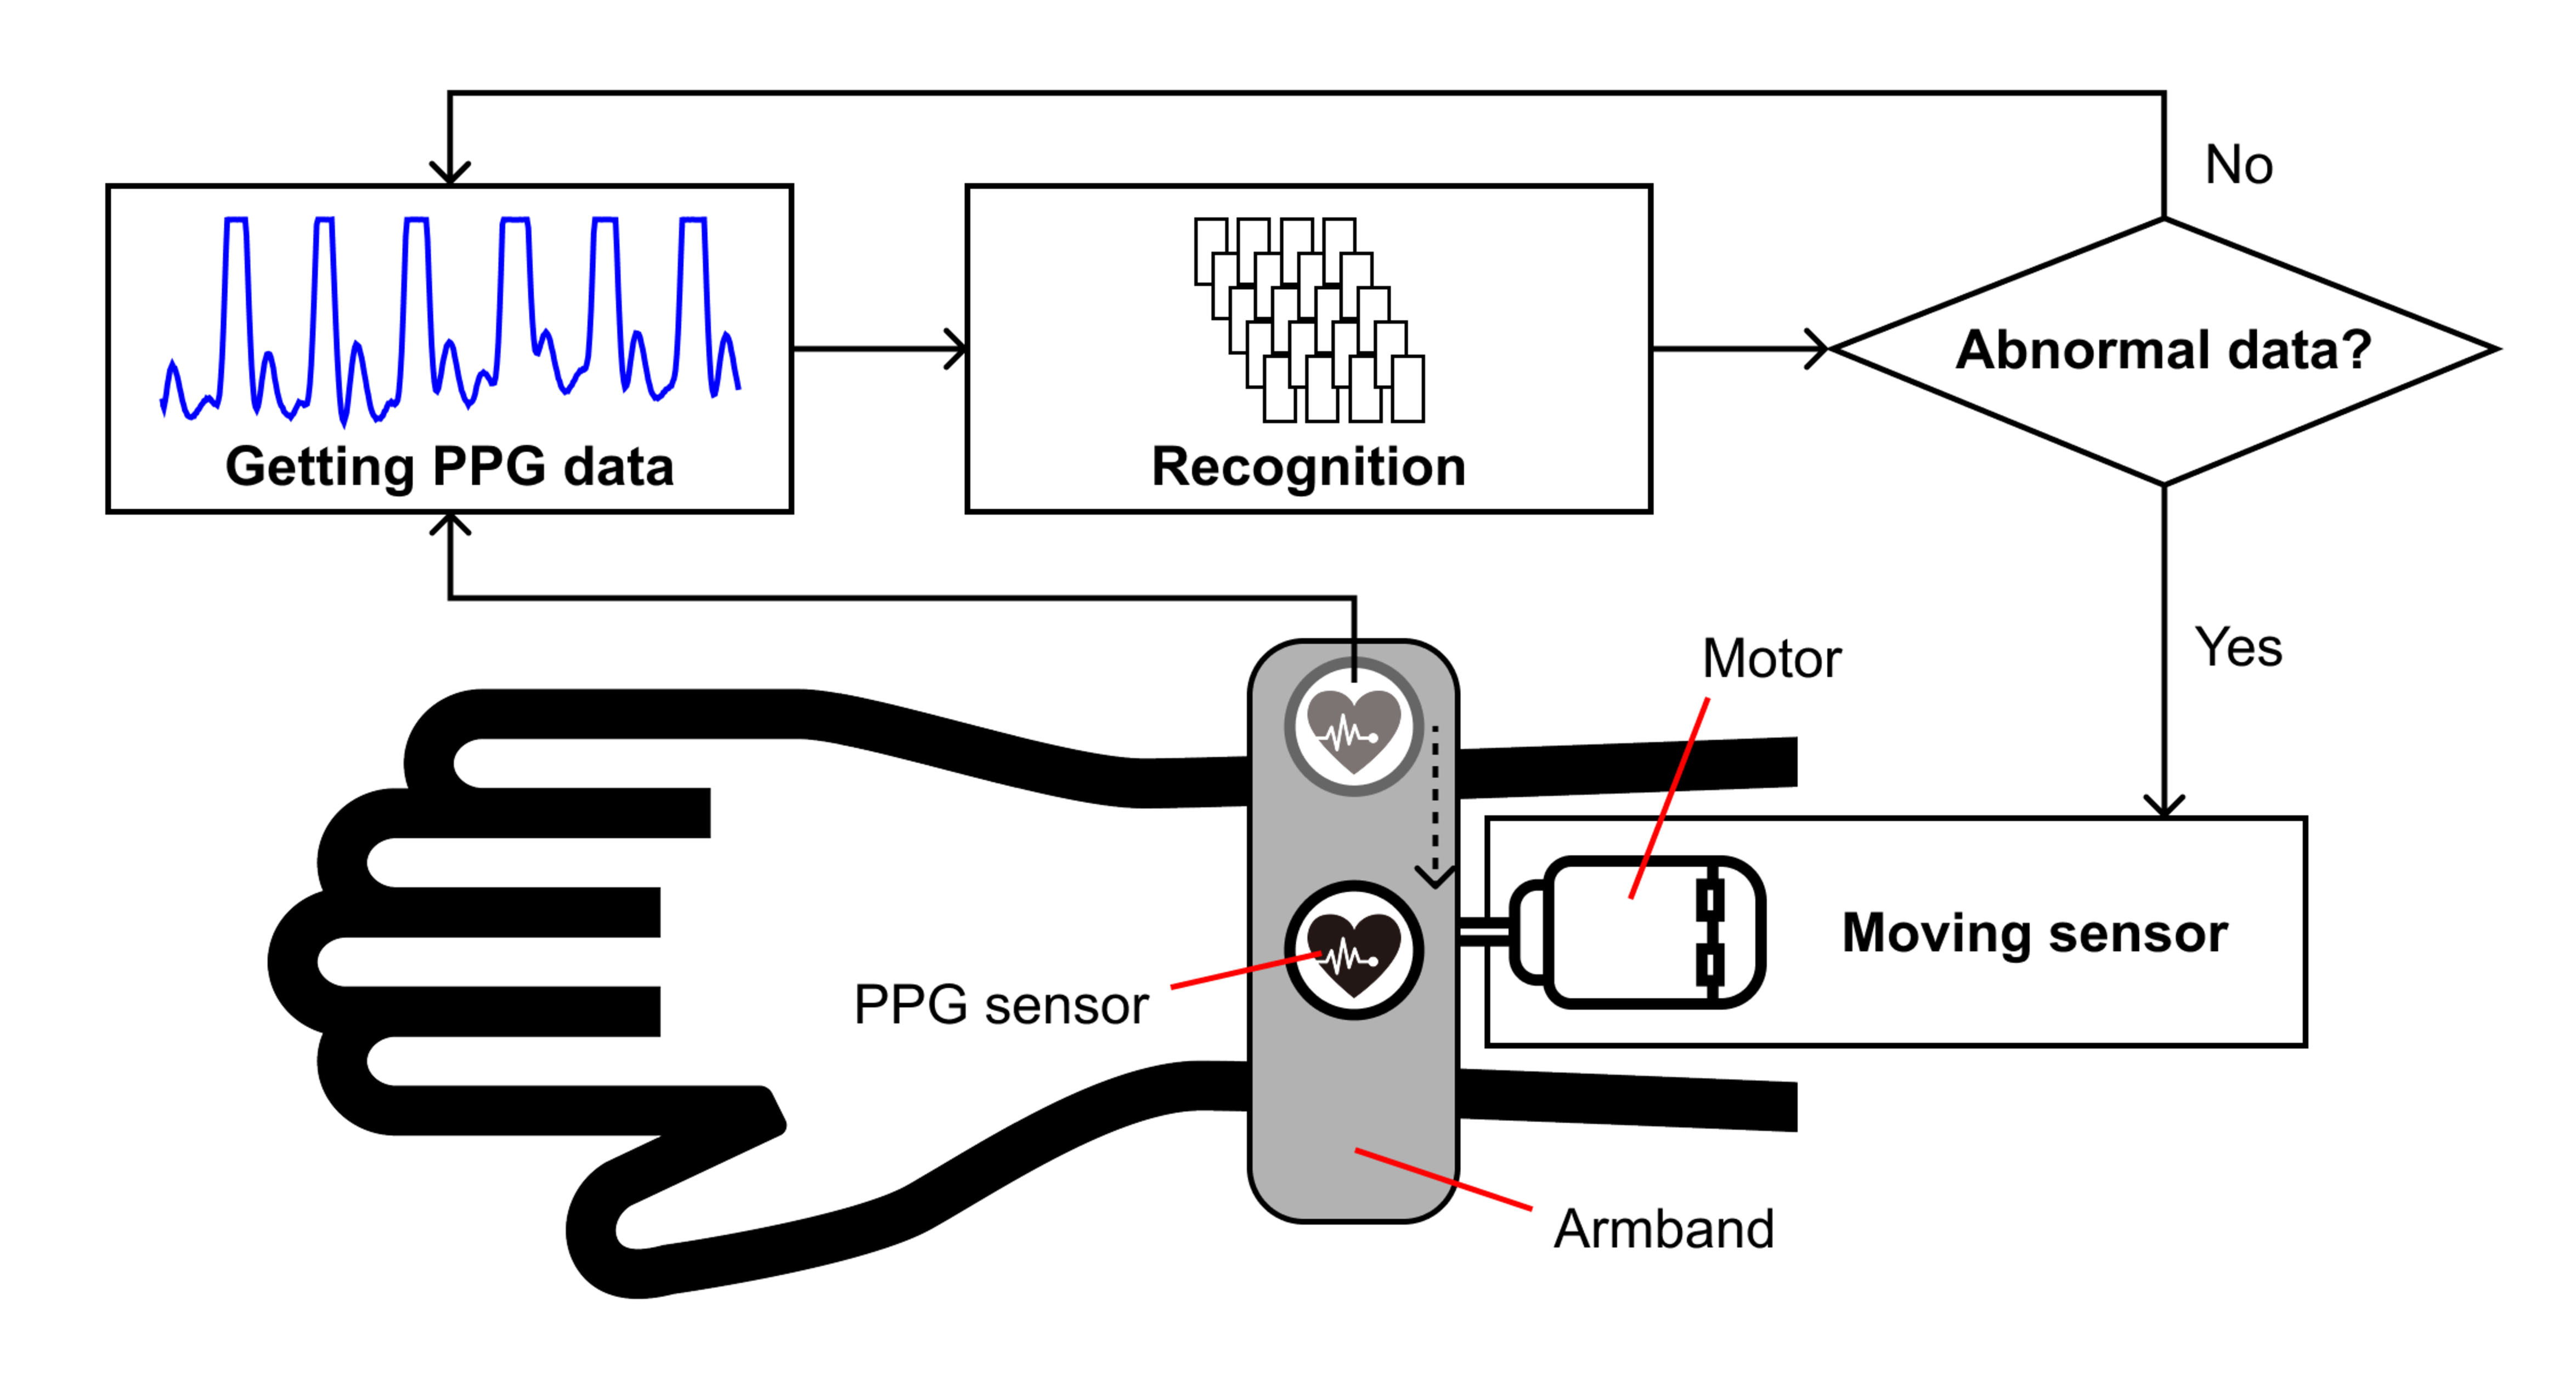
\includegraphics[width=1\linewidth]{figures/system.eps}
  \caption{Process flow of proposed system.}
  \label{fig:system}
\end{figure}


% 3.2
\subsection{Device}
% デバイスを図\figref{device}に、装着した状態を図\figref{waring}に示す。デバイスは駆動部分、制御部分から構成されている。制御部分はモータ、タイミングプーリ、アイドラープーリ、歯付ベルト、PPGセンサが含まれる。制御部分はArduino Uno R3とモータドライバとしてL298Nモジュールを使用している。なお、外部電源はDC12V/1Aを使用している。PPGセンサのデータはArduinoのAnalog A0ピンから取得され、シリアル通信でラップトップへ送られる。ラップトップ上で事前学習された識別モデルへPPGデータを投入し、その識別結果によりモータを作動させる。モータはArduinoのDigital 2, 3ピンにそれぞれHIGH (5V), LOW (0V)の電圧をかけることで作動する。逆電位を設定すると逆方向に回転し、両方のピンをHIGHと設定すると回転にブレーキがかかる。
The device and the mounted state is shown in \figref{device} and \figref{waring}. This consists of a driving unit and a controling unit. The driving unit includes a motor, driving pulley, idler pulley, toothed belt, and PPG sensor. The controling unit includes Arduino Uno R3 microcomputer and L298N module as motor driver. The data from the PPG sensor is obtained from Analog A0 pin on the Arduino and sent to the laptop via serial communication. The PPG data is fed into a pre-trained recognition model on the laptop, and the motor is activated based on the recognition result. The motor is rotate by applying HIGH (5V) and LOW (0V) voltage to the Digital 2 and 3 pins on the Arduino, respectively. Setting the reverse potential will cause the motor to rotate in the opposite direction, and setting both pins HIGH will apply a brake.

\begin{figure}[!t]
  \centering
  \includegraphics[width=1\linewidth]{figures/device.eps}
  \caption{Implemented prototype device.}
  \label{fig:device}
\end{figure}

\begin{figure}[!t]
  \centering
  \includegraphics[width=0.6\linewidth]{figures/waring.eps}
  \caption{The device is worn on the arm.}
  \label{fig:waring}
\end{figure}



% 4
\section{Evaluation}
\label{sec:evaluation}
% 我々は実装したプロトタイプデバイスを使用して、PPGセンサを移動させたときに取得されるデータがどのように変化するかを観察することで提案手法の有効性の評価を行った。
We evaluated the effectiveness of the proposed method with observing how the data acquired changes when the PPG sensor is moved by the implemented prototype device.

% 4.1
\subsection{Data Collection}
% PPGセンサを左手首部分(スマートウォッチを装着するあたり)に装着してデータを収集した。センサを普通に装着した場合と、デバイス越しにセンサを装着した場合の2状態で収集した。データはサンプリングレート約82Hzで15秒間収集された。センサを普通に装着した場合の収集は次のように行った。まず、図\figref{position}の1. topの位置にバンドを用いてセンサを装着し、その状態でデータを収集する。このとき、スマートウォッチの装着を真似て、バンドを軽めに巻いて装着する。次に、バンドを巻いたままの状態で、右手でセンサを2. middleの位置へ移動し、データを収集する。最後に、3. bottomの位置へ移動して、再びデータを収集する。デバイス越しにセンサを装着した場合の収集は同日に実施し、次のように行った。まず、1. topの位置にセンサが設置されるようにデバイスを装着し、その状態でデータを収集する。次に、デバイスを装着したままモータを作動させ、2. middleの位置にセンサを移動させ、停止状態でデータを収集する。最後に、3. bottomの位置へ移動して、再びデータを収集する。なお、比較のための正常な波形として、指先からの同期間のPPGデータも収集した。
The data was collected with the PPG sensor worn on the left wrist area (around where the smartwatch is worn). That collected for 15 seconds at a sampling rate of approximately 82 Hz in two states: with the sensor worn normally and with the sensor worn over the device. The collection when the sensor was worn normally was conducted as follows. First, the sensor was attached using a band at ``1. Top'' position in \figref{position}, and the data was collected. At this point, the band was lightly fasten to mimic the wearing of a smartwatch. Next, the sensor was moved to ``2. Middle'' position by the right hand without removing the band, and the data was collected. Finally, the sensor was moved to ``3. Bottom'' position, and the collection was conducted again. The collection of the sensor worn over the device was conducted on the same day and was done as follows. First, the device is worn so that the sensor is mounted at ``1. Top'' position, and the data was collected. Next, the motor was rotated with the device in place. The sensor was moved to ``2. Middle'' position, and the data was collected after the motor was stopped. Finally, the data was collected at ``3. Bottom'' position with the same process. The PPG data of the same time from the finger were also collected as normal waveforms for comparison.

\begin{figure}[!t]
  \centering
  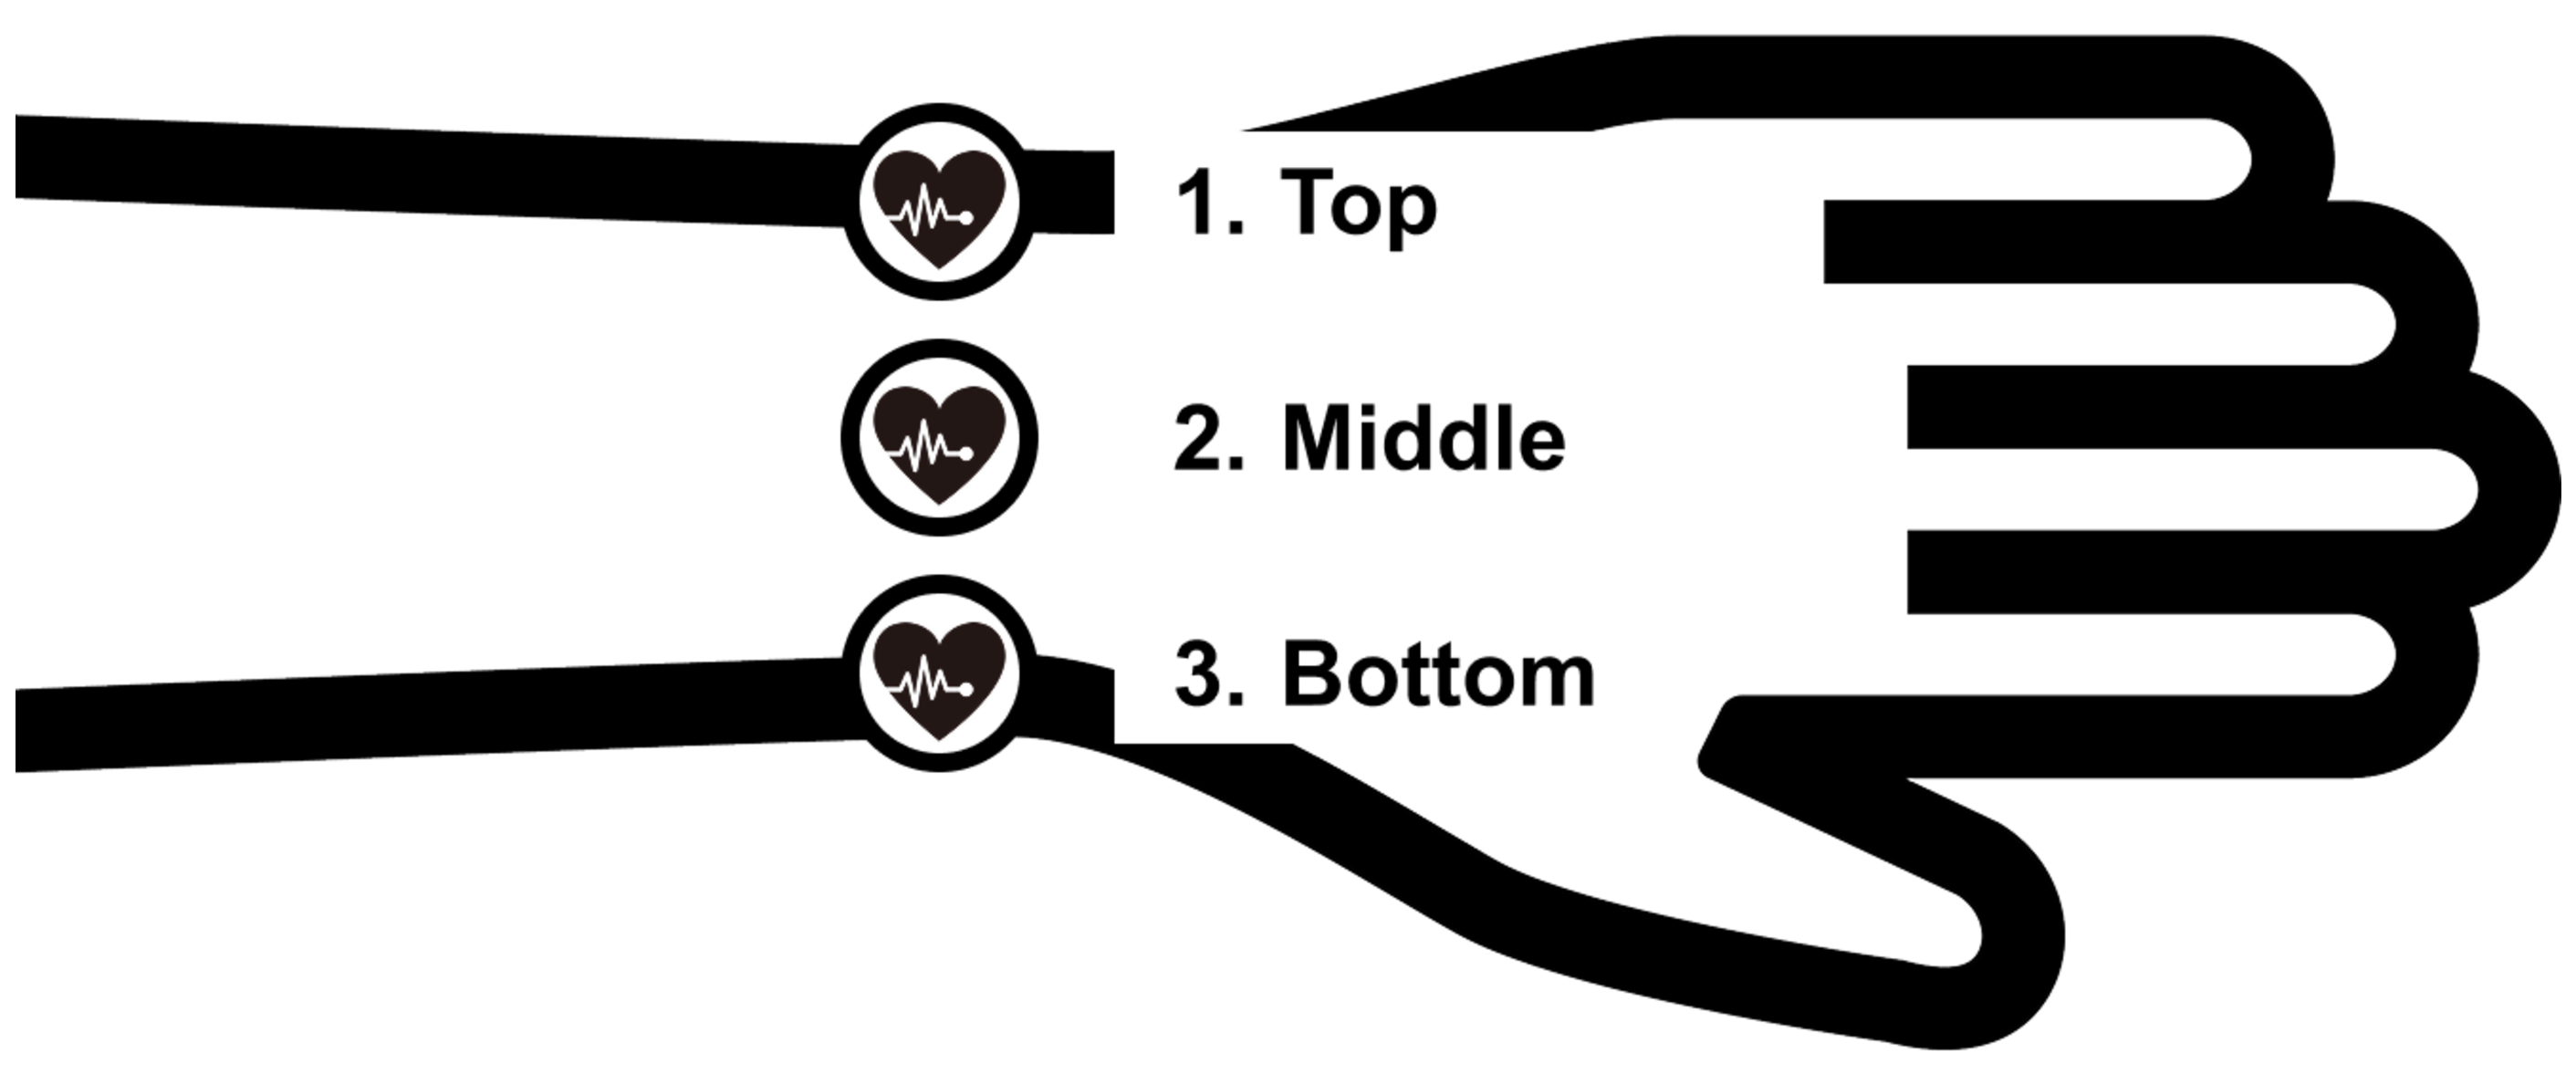
\includegraphics[width=0.7\linewidth]{figures/position.eps}
  \caption{Mounting position of the sensor.}
  \label{fig:position}
\end{figure}


% 4.2
\subsection{Environment for Evaluation Experiments}
% 収集されたデータのうち最初の5秒間はキャリブレーション期間とし、後半の10秒間のデータを分析に使用した。データの質を分析するために、生データからピーク検出を行った。ピーク検出は心拍数の計測に使用される。我々は、事前収集したデータに対し、SciPyのfind_peaksを使用してピーク検出を行った。ピーク同士の最小間隔であるdistanceパラメータは50を設定した。また、我々は正常脈波(指先から)と腕からの脈波の類似度を確認するために,DTWアルゴリズムを使用して波形同士のL1ノルムを計算した。
The first 5 seconds of the collected data were discarded as a calibration period, and only the latter 10 seconds of data were used for analysis. We performed peak detection was performed from the raw data to analyze data quality. Peak detection is used to measure heart rate. \texttt{scipy.signal.find\_peaks}\footnote{\url{https://docs.scipy.org/doc/scipy/reference/generated/scipy.signal.find_peaks.html}} of SciPy\footnote{\url{https://scipy.org/}} was used to perform peak detection to the pre-collected data. The distance parameter which is the minimum distance between peaks was set to 50. We also calculated the L1 norm between normal pulse waves (from finger) and those from the arm using the DTW algorithm to check the similarity.


% 4.3
\subsection{Results and Discussion}
% PPGセンサは装着位置により取得されるデータが変化するほか、心拍数は常に変化しているため、同じ日に収集したとしても全く同じ波形のデータを取得することはできない。そのため、通常の装着とデバイス上での装着の場合で、腕と指先の脈波の差が変化するかどうかを確認する。
The PPG sensor cannot acquire exactly the same data even if it is collected on the same day, because the data acquired varies depending on the wearing position and the heart rate is constantly changing. Therefore, we evaluated whether the difference in waveform between the arm and finger changes when the sensor is worn normally and over the device.\par

% 収集されたPPGデータの波形を図\figref{manual}、図\figref{auto}に示す。検出されたピークは点で示されている。波形から、指先から取得されたデータに比べて、腕から取得されたデータは振幅が小さく特徴が見えにくいことがわかる。しかしながら、これはデバイス上のPPGセンサからのデータだけでなく、通常の装着をしたセンサからのデータでも同じ結果であるため、本デバイスによる影響ではないことがわかる。我々は指先に比べて腕は皮膚が厚く、血管が浮き出ていないため、フォトリフレクタが反射光を十分に捉えられなかったことが影響したと考えている。
The waveform of collected PPG data are shown in \figref{manual} and \figref{auto}. The detected peaks are indicated by dots. It can be seen that the data acquired from the arm has smaller amplitudes and features are less visible compared to the data acquired from the finger. However, this is not an effect of this device, since this result is the same not only for the data from the PPG sensor on the device, but also for the data from the sensor with normal wear. We think that this result is due to the fact that the skin of the arm is thicker than that of the fingertips, which means that the blood vessels do not appear, and the phototransistor did not capture enough reflected light.\par

% 検出されたピーク数と、計算されたDTW距離を表\tabref{manual}, 表\tabref{auto}に示す。腕と指先の脈波のピーク数は2回以内の差であり、デバイスの利用により大きな差が発生することはなかった。また、DTW距離に関しては、Top, Middle, Bottomの順に小さくなる結果となった。デバイスの利用により順位が入れ替わることはなかった。
The number of peaks detected and the calculated DTW distances are shown in \tabref{manual} and \tabref{auto}. The number of peaks for the arm and finger differed within 2 times, and no significant differences were caused by the use of the device. The DTW distance was smaller in the order of Top, Middle, and Bottom. The order did not change depending on the use of the device.\par

% この結果から、手動でPPGの位置を調整しても、デバイスを使って位置を調整しても取得されるデータに差は発生しないということが明らかになった。そのため、PPGデータが異常波形になった場合、デバイスにより正常波形が取得できる位置にセンサを移動させる本手法は有効であると考えている。
The results indicate that there is no difference in the data acquired when the PPG position is manually adjusted or when the position is adjusted using a device. Therefore, the proposed method of moving the sensor to a position where a normal waveform can be acquired by the device is effective when the PPG data has an abnormal waveform.

\begin{figure*}[!t]
  \centering
  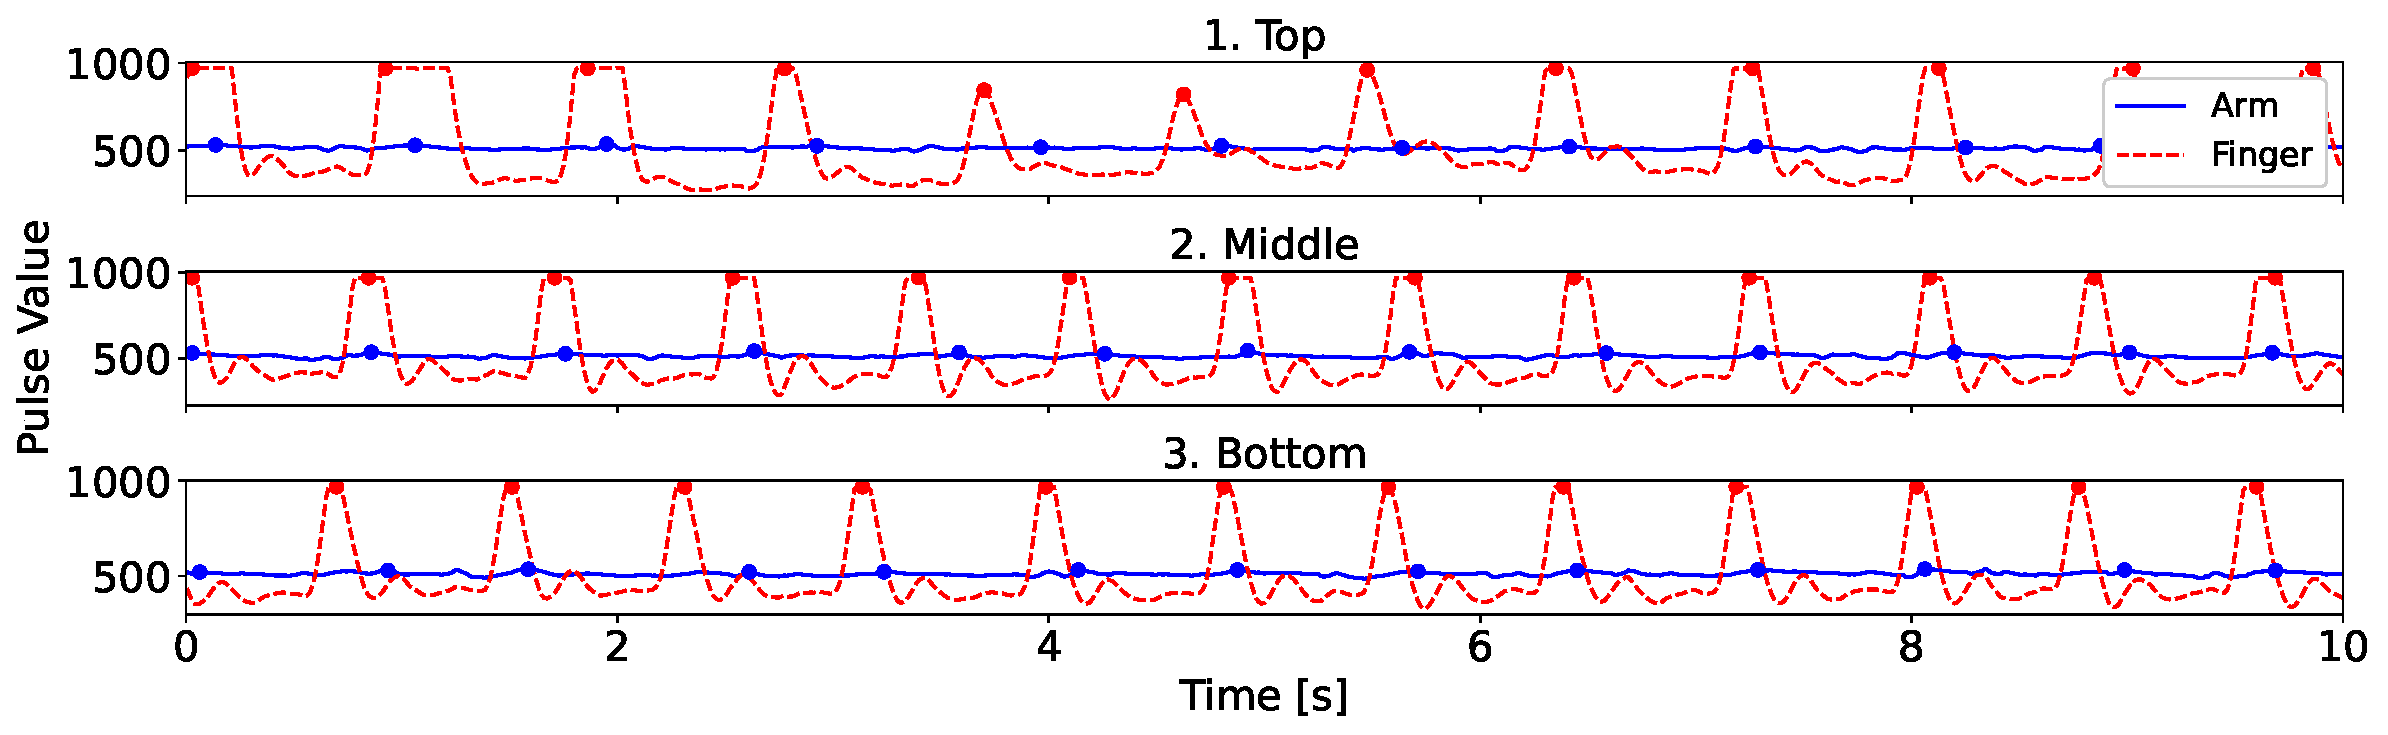
\includegraphics[width=1\linewidth]{figures/manual.eps}
  \caption{Confusion matrix in bottle estimation.}
  \label{fig:manual}
\end{figure*}

\begin{figure*}[!t]
  \centering
  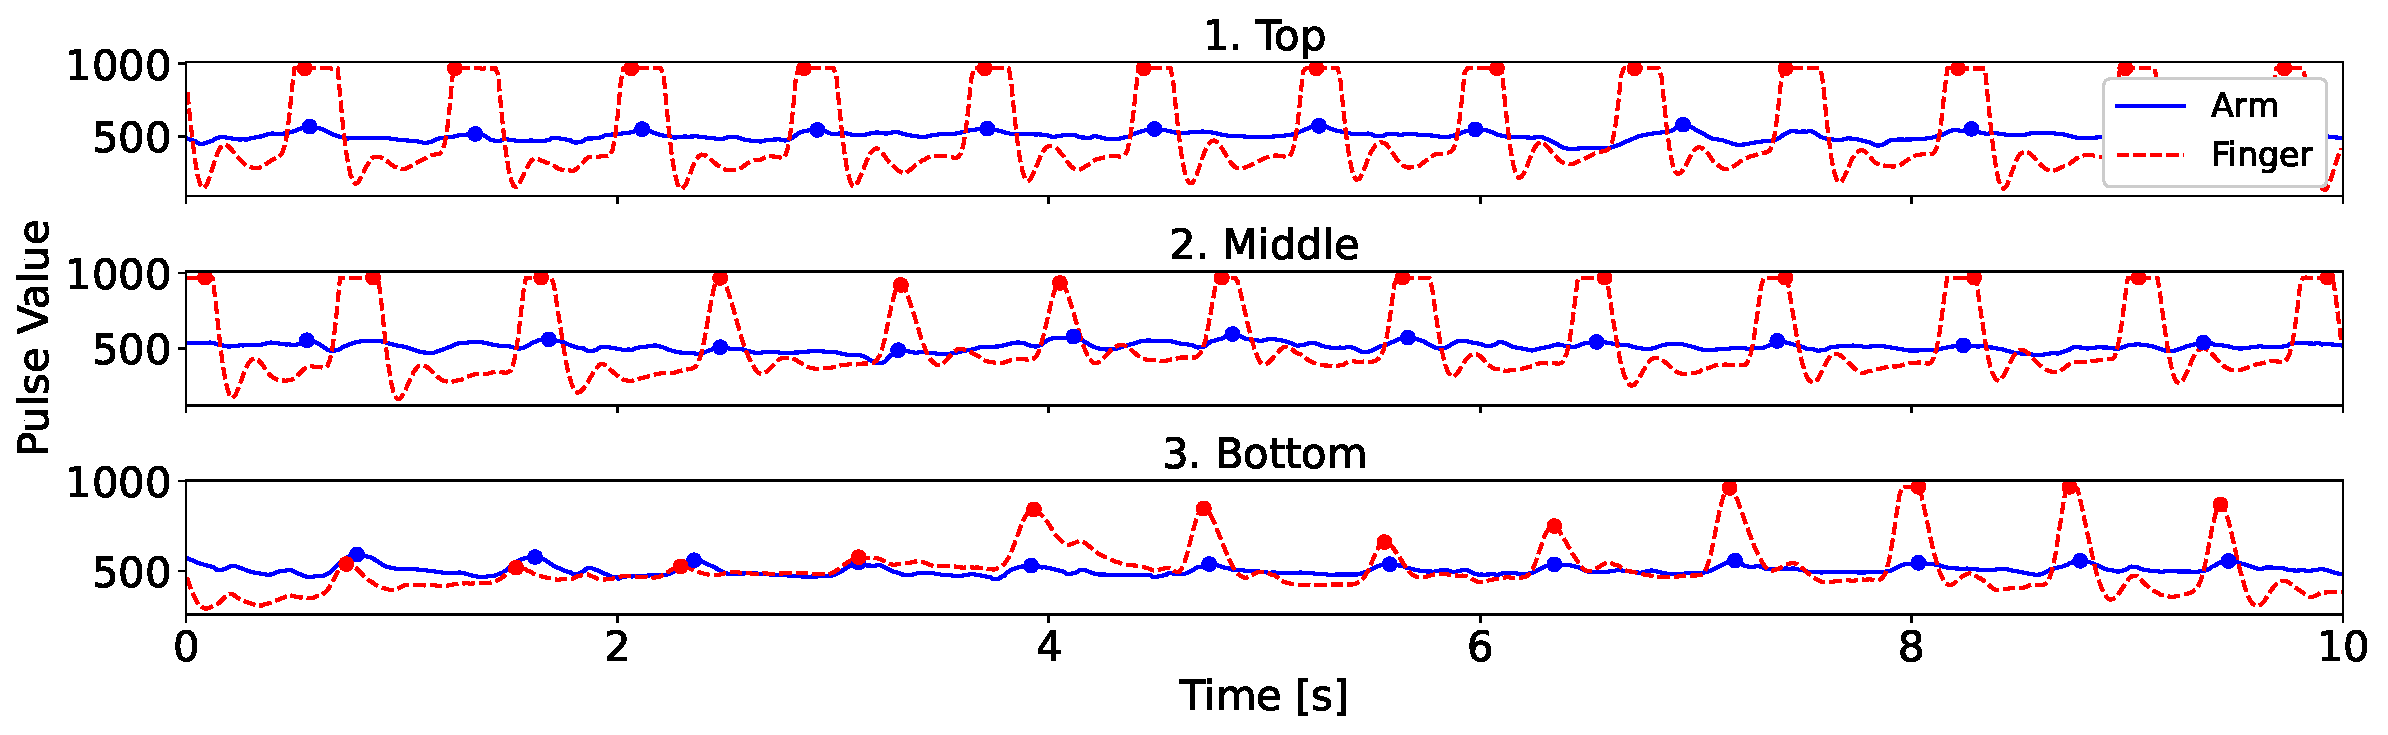
\includegraphics[width=1\linewidth]{figures/auto.eps}
  \caption{Change in loss during training phase of bottle estimation model.}
  \label{fig:auto}
\end{figure*}

\begin{table}[!t]
  \small
  \centering
  \caption{Number of peaks and DTW distance in PPG data when the sensor is worn normally.}
  \begin{tabular}{c|c|cc|c} \hline\hline
    \multirow{2}{*}{\#} & \multirow{2}{*}{Position} & \multicolumn{2}{c|}{Peaks} & \multirow{2}{*}{DTW distance} \\ \cline{3-4}
     &                   & Arm & Finger & \\ \hline
    1 & Top & 12 & 12 & 142840 \\
    2 & Middle & 13 & 13 & 130004 \\
    3 & Bottom & 13 & 12 & 104028 \\ \hline
  \end{tabular}
  \label{tab:manual}
\end{table}

\begin{table}[!t]
  \small
  \centering
  \caption{Number of peaks and DTW distance in PPG data when the sensor is worn over the device.}
  \begin{tabular}{c|c|cc|c} \hline\hline
    \multirow{2}{*}{\#} & \multirow{2}{*}{Position} & \multicolumn{2}{c|}{Peaks} & \multirow{2}{*}{DTW distance} \\ \cline{3-4}
     &                   & Arm & Finger & \\ \hline
    1 & Top & 12 & 13 & 174512 \\
    2 & Middle & 11 & 13 & 130848 \\
    3 & Bottom & 12 & 12 & 56261 \\ \hline
  \end{tabular}
  \label{tab:auto}
\end{table}



% 5
\section{Future Work}
\label{sec:future_work}
% 評価実験の結果、デバイスを使用してPPGセンサの装着位置を調整しても、正常なデータを取得できることが明らかになった。今後は、PPGデータが正常な波形か異常な波形かを識別するモデルを構築していく。リアルタイムにPPGデータを取得し、異常な波形を検知することが可能となれば、本論文にて実装したプロトタイプデバイスのモータ制御処理に組み込んでいく。そして、正常な脈波データを継続的に取得できるかどうかの評価実験を行う予定である。
The results of the evaluation experiment showed that normal data can be obtained even when the device is used to adjust the mounting position of the PPG sensor. In the future, we will implement a model to recognize whether PPG data is normal or abnormal waveforms. If it becomes possible to acquire data in real time and detect abnormal waveforms, we will incorporate it into the motor control of the prototype device implemented in this paper. Then, we plan to conduct evaluation experiments to see if normal pulse data can be continuously acquired.\par

% また、現状のデバイスはサイズが大きい。またセンサの移動が直線方向となっており、腕の曲面部分にセンサを設置することができない。実際の使用を想定して、腕に装着することが可能なようにデバイスの改良を進めていく。
In addition, current devices are large in size. The sensor moves in a straight line, making it impossible to place the sensor on the curved surface of the arm. We will continue to improve the device so that it can be worn on the arm for real-world use.



% 6
\section{Conclusion}
\label{sec:conclution}
% 本論文では、センサが異常な脈波データを検出した時に、センサを移動させて装着部位を調整するデバイスを提案しました。
% In this paper, we proposed a method to estimate the water level in a container by acquiring the sound of water pouring, assuming a device attached to a faucet, so that the water level can be correctly determined even in a container whose internal conditions are difficult to grasp. We implemented several estimation models and conducted experiments to evaluate the estimation accuracy using five bottles. The results showed that the bottle estimation model had an average accuracy of 0.642, the water level estimation model had respective averages of 0.462 and 0.308 for the bottle-dependent and bottle-independent models, and the overflow detection model had respective averages of 0.83 and 0.744 for the bottle-dependent and bottle-independent models. These results indicate that, while the accuracy of the water level estimation needs to be improved, overflow detection can be achieved regardless of the container type and may be used in natural environments. In the future, we plan to improve the model for better estimation accuracy and to implement a faucet-mounted device that incorporates a function to stop water injection just before it becomes full.

%%
%% The acknowledgments section is defined using the "acks" environment
%% (and NOT an unnumbered section). This ensures the proper
%% identification of the section in the article metadata, and the
%% consistent spelling of the heading.
% \begin{acks}
% To Robert, for the bagels and explaining CMYK and color spaces.
% \end{acks}

%%
%% The next two lines define the bibliography style to be used, and
%% the bibliography file.
\bibliographystyle{ACM-Reference-Format}
\bibliography{references}


%%
%% If your work has an appendix, this is the place to put it.
% \appendix

% \section{Research Methods}

% \subsection{Part One}

% Lorem ipsum dolor sit amet, consectetur adipiscing elit. Morbi
% malesuada, quam in pulvinar varius, metus nunc fermentum urna, id
% sollicitudin purus odio sit amet enim. Aliquam ullamcorper eu ipsum
% vel mollis. Curabitur quis dictum nisl. Phasellus vel semper risus, et
% lacinia dolor. Integer ultricies commodo sem nec semper.

% \subsection{Part Two}

% Etiam commodo feugiat nisl pulvinar pellentesque. Etiam auctor sodales
% ligula, non varius nibh pulvinar semper. Suspendisse nec lectus non
% ipsum convallis congue hendrerit vitae sapien. Donec at laoreet
% eros. Vivamus non purus placerat, scelerisque diam eu, cursus
% ante. Etiam aliquam tortor auctor efficitur mattis.

% \section{Online Resources}

% Nam id fermentum dui. Suspendisse sagittis tortor a nulla mollis, in
% pulvinar ex pretium. Sed interdum orci quis metus euismod, et sagittis
% enim maximus. Vestibulum gravida massa ut felis suscipit
% congue. Quisque mattis elit a risus ultrices commodo venenatis eget
% dui. Etiam sagittis eleifend elementum.

% Nam interdum magna at lectus dignissim, ac dignissim lorem
% rhoncus. Maecenas eu arcu ac neque placerat aliquam. Nunc pulvinar
% massa et mattis lacinia.

\end{document}
\endinput
%%
%% End of file `sample-sigconf-authordraft.tex'.
